\section{Experiment 1}
In this experiment we would like to test the elasticity and how the area of the beam is preserved when applying varying amounts of force to different materials. We will look at the materials steel, glass, rubber and lead. As our model makes assumptions about small displacements, and all material wants to return to its original shape, we will expect no loss and no gain in area when we apply force. Beginning with steel we can visualize the displacement when applying $-10^7$ units of force to each node along with a plot of the area of the beam when different amounts of force is applied. The results can be seen in \autoref{steel}.
\begin{figure}[H]
	\centering
	\begin{subfigure}[b]{0.49\linewidth}
		\centering
		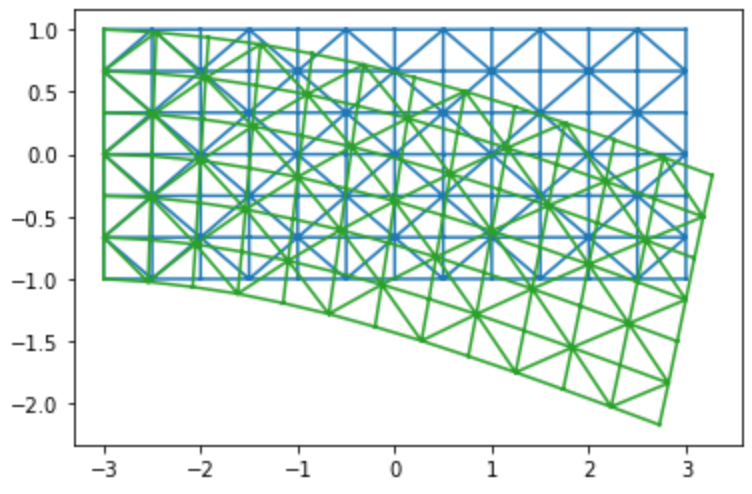
\includegraphics[width=\linewidth]{Materials/Steelviz}
		\caption{$-10^7$ units of force applied to steel.\\\hfill}
	\end{subfigure}
	\hfill
	\begin{subfigure}[b]{0.49\linewidth}
		\centering
		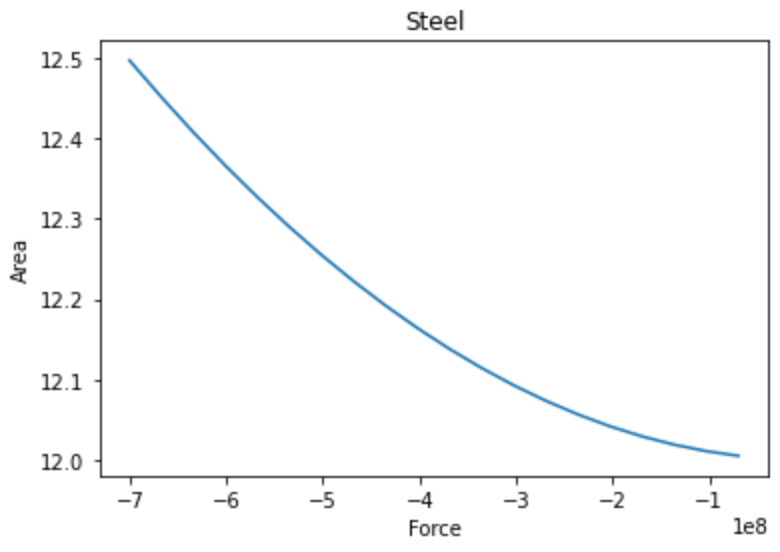
\includegraphics[width=\linewidth]{Materials/SteelArea}
		\caption{Relation between force and area for steel.}
	\end{subfigure}
	\caption{Example of steel displacement together with relation between force and area for steel. Young's modulus is $69^9$ and Poisson ratio is $0.3$.}
	\label{steel}
\end{figure}
We see that the increase in area is somewhat significant and exponentially increasing. Looking at how the bar deforms, we see the topline of the right side not bending, but instead the middle of the bar bending. We can now look at glass which have surprisingly similar Young's modulus and Poisson ratio. The results can be seen in \autoref{glass}.
\begin{figure}[H]
	\centering
	\begin{subfigure}[b]{0.49\linewidth}
		\centering
		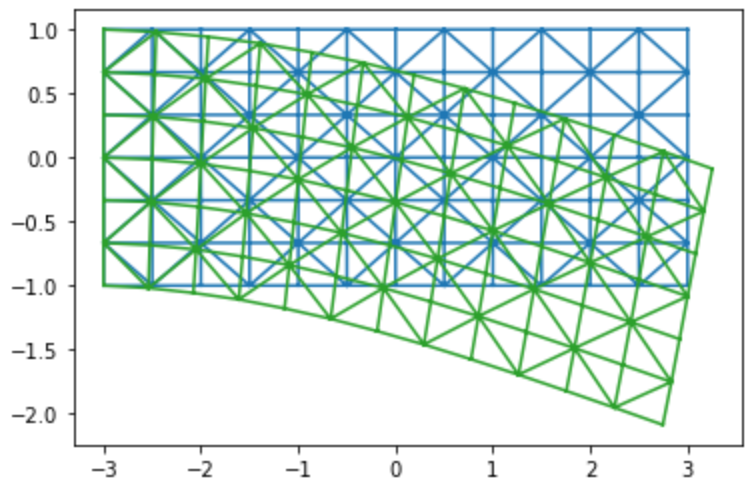
\includegraphics[width=\linewidth]{Materials/Glassviz}
		\caption{$-10^7$ units of force applied to glass.}
	\end{subfigure}
	\hfill
	\begin{subfigure}[b]{0.49\linewidth}
		\centering
		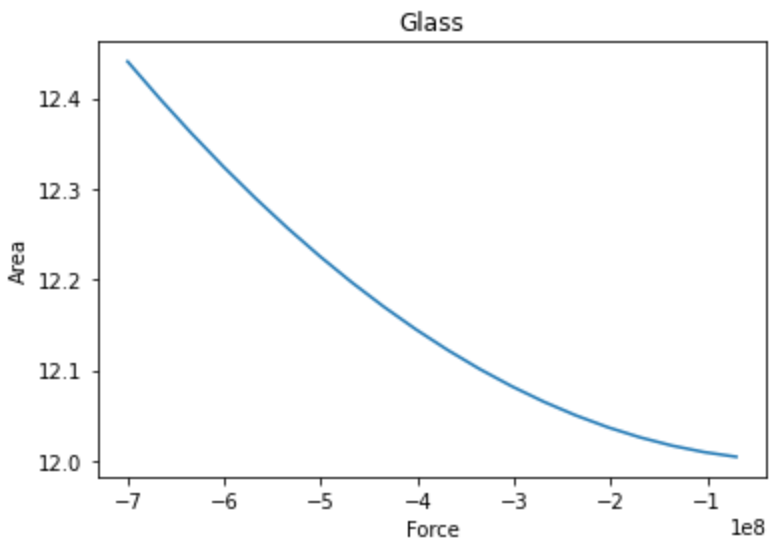
\includegraphics[width=\linewidth]{Materials/GlassArea}
		\caption{Relation between force and area for glass.}
	\end{subfigure}
	\caption{Example of glass displacement together with relation between force and area for steel. Young's modulus is $70^9$ and Poisson ratio is $0.22$.}
	\label{glass}
\end{figure}
We here see similar results where the area changes exponentially, but slightly less than for steel and the beam bends in a natural way. Looking at rubber we have a big decrease in Young's modulus and big increase in Poisson ratio. The results can be seen in \autoref{rubber}.
\begin{figure}[H]
	\centering
	\begin{subfigure}[b]{0.49\linewidth}
		\centering
		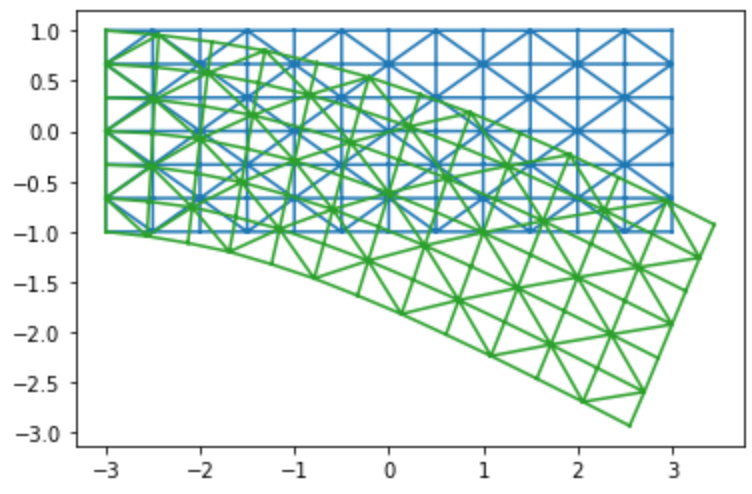
\includegraphics[width=\linewidth]{Materials/Rubberviz}
		\caption{$-10^4$ units of force applied to rubber.}
	\end{subfigure}
	\hfill
	\begin{subfigure}[b]{0.49\linewidth}
		\centering
		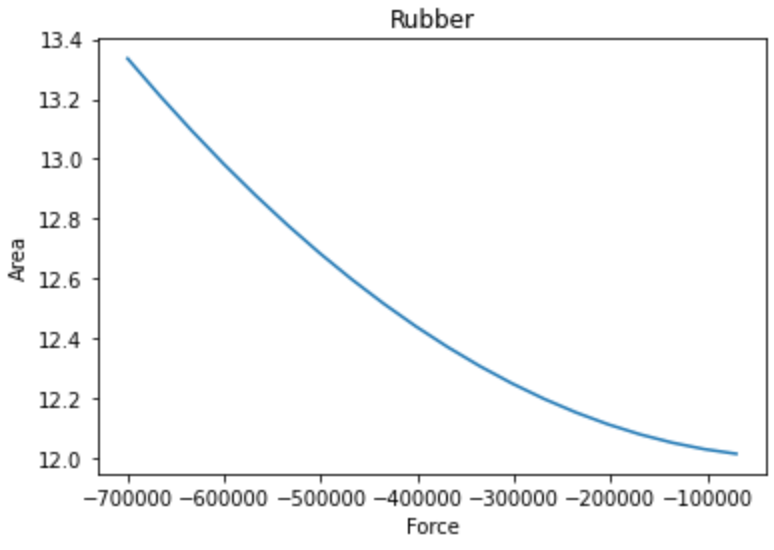
\includegraphics[width=\linewidth]{Materials/RubberArea}
		\caption{Relation between force and area for rubber.}
	\end{subfigure}
	\caption{Example of rubber displacement together with relation between force and area for steel. Young's modulus is $0.05^9$ and Poisson ratio is $0.49$.}
	\label{rubber}
\end{figure}
We here note we need a lot less force to bend the beam, but we still see the same results, exponential increase in area, and the beam bending in a natural way. The last material we will look at is lead and the results can be seen in \autoref{lead}.
\begin{figure}[H]
	\centering
	\begin{subfigure}[b]{0.49\linewidth}
		\centering
		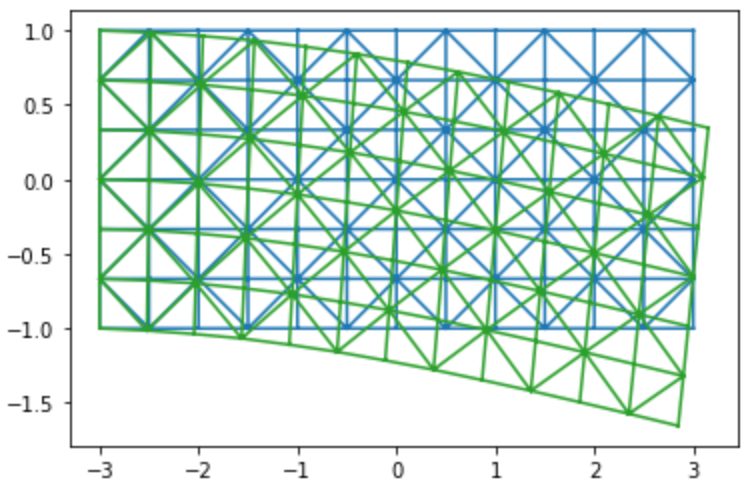
\includegraphics[width=\linewidth]{Materials/Leadviz}
		\caption{$-10^6$ units of force applied to lead.\\\hfill}
	\end{subfigure}
	\hfill
	\begin{subfigure}[b]{0.49\linewidth}
		\centering
		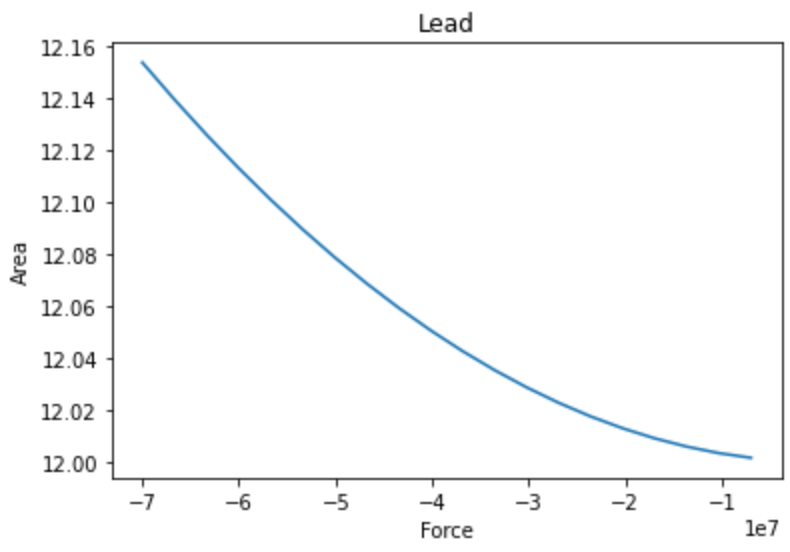
\includegraphics[width=\linewidth]{Materials/LeadArea}
		\caption{Relation between force and area for lead.}
	\end{subfigure}
	\caption{Example of lead displacement together with relation between force and area for steel. Young's modulus is $13.8^9$ and Poisson ratio is $0.431$.}
	\label{lead}
\end{figure}
We again see a natural bend and exponential increase in area.

\subsection{Discussion of results}
For all material we see an exponential increase in area as we apply force to the beams. As we expected no change in area, we thus conclude our model does introduce some amount of error into our simulation. We can also rank the materials after which we would expect would require the most force to bend. Here We would properly expect steel to require the most force to bend. However, the results shows we need approximately the same force to bend steel and glass. As Young's modulus and Poisson ratio for the two materials are quite close, this is not too surprising. However, I have chosen to go with the assignment value for Young's modulus on steel although some websites put much higher, making steel harder to bend, which would put it in line with our expectation. As we would expect, rubber is the easiest of the four materials to bend, and lead comes in third. The fact the model concurs with our expectation, we conclude we have verified that the model works correctly in this regard.